% !TeX spellcheck = cs_CZ
\wikitextrule
\begin{example}\label{mai:exam004}
  \textbf{Parametrická vyjádření roviny}:\newline\small
  Rovina v trojrozměrném prostoru \(\mathbb{R}^3\) je zadána třemi body \(A\), \(B\) a \(C\), 
  které nesmějí ležet v jedné přímce, popřípadě dvěma body \(A\) a \(B\) a vektorem \(\vec{v}\) 
  nerovnoběžným s \(\overrightarrow{AB}\), anebo bodem \(A\) a dvěma nerovnoběžnými směrovými 
  vektory \(\vec{u}\) a \(\vec{u}\) (obr. \ref{MAI:FIG002}). Všechny tyto typy zadání jsou 
  ekvivalentní. Lze volit například \(\vec{u} = \overrightarrow{AB}\), \(\vec{v} = 
  \overrightarrow{AC}\). Je-li \(X\) libovolným bodem roviny \(\varrho\), jsou vektory 
  \(\overrightarrow{AX}\), \(\vec{u}\) a \(\vec{v}\) \textbf{lineárně závislé}. To znamená, že 
  existují taková reálná čísla \(r\) a \(s\), že vektor \(\overrightarrow{AX}\) lze zapsat jako 
  lineární kombinaci

  {\centering
    \captionsetup{type=figure}
    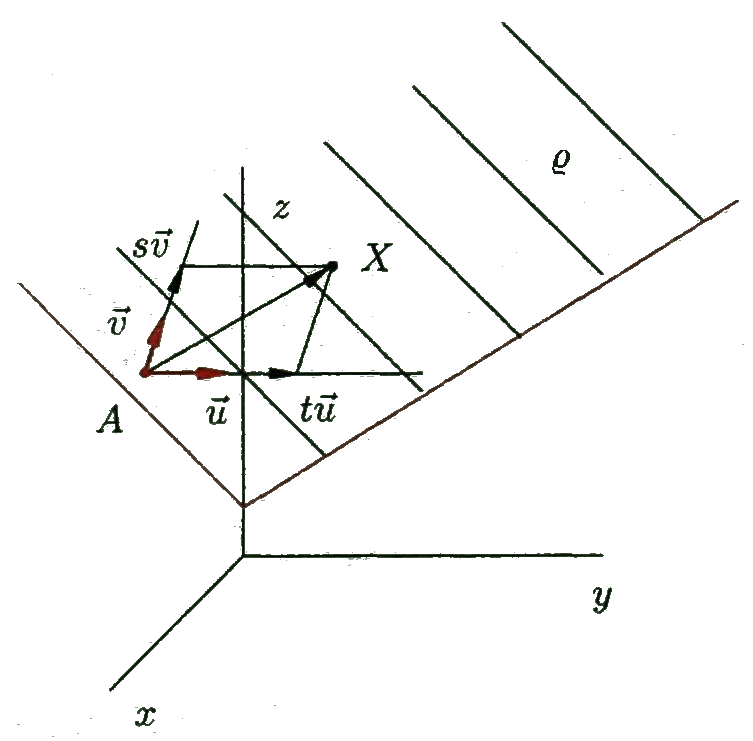
\includegraphics[width=0.4\linewidth]{mai_fig026.png}
    \captionof{figure}{Zadání roviny. \cite[s.~3]{Musilova2009MA1}
    \label{MAI:FIG002}}
    \par}
  
  \begin{equation*}
    \overrightarrow{AX} = r\cdot\vec{u} + s\cdot\vec{v}, \qquad r,s \in\mathbb{R}
  \end{equation*}
  Při obdobném zápisu kartézských souřadnic bodů a složek vektorů jako u vyjádření přímky dostaneme
  parametrické vyjádření roviny \(\varrho\)
  \begin{equation}\label{mai:eq039}
    \varrho = \left\{(x,y,z)\in\mathbb{R}^3\,|\,
    \begin{matrix}
      x = x_A + ru_1 + sv_1,        \\
      y = y_A + ru_2 + sv_2,        \\
      z = z_A + ru_3 + sv_3,
    \end{matrix}
    \;r,s\in\mathbb{R}
    \right\}.
  \end{equation}
  Toto vyjádření obsahuje opět lineární závislost: Souřadnice \(x\), \(y\) a \(z\) se vůči 
  souřadnicím bodu \(A\) mění v závislosti na prvních mocninách parametrů \(r\) a \(s\). Můžeme tak 
  hovořit o jakési „vícerozměrné úměře“.
  \normalsize
\end{example}
  